%% Based on a TeXnicCenter-Template by Gyorgy SZEIDL.
%%%%%%%%%%%%%%%%%%%%%%%%%%%%%%%%%%%%%%%%%%%%%%%%%%%%%%%%%%%%%

%------------------------------------------------------------
%
\documentclass{article}%
%Options -- Point size:  10pt (default), 11pt, 12pt
%        -- Paper size:  letterpaper (default), a4paper, a5paper, b5paper
%                        legalpaper, executivepaper
%        -- Orientation  (portrait is the default)
%                        landscape
%        -- Print size:  oneside (default), twoside
%        -- Quality      final(default), draft
%        -- Title page   notitlepage, titlepage(default)
%        -- Columns      onecolumn(default), twocolumn
%        -- Equation numbering (equation numbers on the right is the default)
%                        leqno
%        -- Displayed equations (centered is the default)
%                        fleqn (equations start at the same distance from the right side)
%        -- Open bibliography style (closed is the default)
%                        openbib
% For instance the command
%           \documentclass[a4paper,12pt,leqno]{article}
% ensures that the paper size is a4, the fonts are typeset at the size 12p
% and the equation numbers are on the left side
%
\usepackage{amsmath}%
\usepackage{amsfonts}%
\usepackage{amssymb}%
\usepackage{graphicx}
\usepackage{tikz}
\usepackage{float}
\usepackage[utf8]{inputenc}
\usepackage{longtable}
\usetikzlibrary {positioning}

%-------------------------------------------
\newtheorem{theorem}{Theorem}
\newtheorem{acknowledgement}[theorem]{Acknowledgement}
\newtheorem{algorithm}[theorem]{Algorithm}
\newtheorem{axiom}[theorem]{Axiom}
\newtheorem{case}[theorem]{Case}
\newtheorem{claim}[theorem]{Claim}
\newtheorem{conclusion}[theorem]{Conclusion}
\newtheorem{condition}[theorem]{Condition}
\newtheorem{conjecture}[theorem]{Conjecture}
\newtheorem{corollary}[theorem]{Corollary}
\newtheorem{criterion}[theorem]{Criterion}
\newtheorem{definition}[theorem]{Definition}
\newtheorem{example}[theorem]{Example}
\newtheorem{exercise}[theorem]{Exercise}
\newtheorem{lemma}[theorem]{Lemma}
\newtheorem{notation}[theorem]{Notation}
\newtheorem{problem}[theorem]{Problem}
\newtheorem{proposition}[theorem]{Proposition}
\newtheorem{remark}[theorem]{Remark}
\newtheorem{solution}[theorem]{Solution}
\newtheorem{summary}[theorem]{Summary}
\newenvironment{proof}[1][Proof]{\textbf{#1.} }{\ \rule{0.5em}{0.5em}}
\def\labelitemi{}

\begin{document}

\title{Science of Information, Statistics, and Learning Lecture $15$} %Change lecture number here
\author{Parmanand Khajuriya 12D070041, Bankuru Dharma Teja 130050049,\\
 Jay Mardia13D070011, Sudipto Mitra 130100014,\\ 
 Sachin Garg 13D070061
}
\date{Mar 17,2017}
\maketitle
 
\begin{abstract}
In the previous lecture, we studied linear regression and spoke about the need to choose a hypothesis class, and given a hypothesis class, to choose an underlying model for generating our data which could motivate the error measure we use to pick the best hypothesis from out hypothesis class. Specifically, we saw that Gaussian measurement noise coupled with wanting to maximize likelihood lead to a square-error. In this lecture, we study the binary classification problem and relate the quantities that arise to Physics and Information Theory. In doing so, we end up studying the single neuron as a classifier.

Most of today's lecture is based on Ch-39 from "Information Theory, Inference, and Learning Algorithms" by David J.C. MacKay
\end{abstract}

\section*{Introduction}
Suppose we are given a bunch of points in an n-dimensional feature space ($\mathbb{R}^n$) with each point labelled by a {Yes, No} or {0,1}.

\begin{figure}[H]
	\centering
		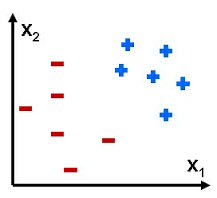
\includegraphics[scale=0.37]{BinaryClassification.png}
   	\caption{A bunch of data points with labels of {Yes,No} represented by [Plus,Minus]}
\end{figure}

\pagebreak
\section{Problem Formulation}
\textbf{Input:}
\newline
$x_1 \in \mathbb{R}^n, t_1 \in \{Yes,No\}$
\newline
$x_2 \in \mathbb{R}^n, t_2 \in \{Yes,No\}$
\newline
$x_3 \in \mathbb{R}^n, t_3 \in \{Yes,No\}$
\newline
.
\newline
.
\newline
$x_N \in \mathbb{R}^n, t_N \in \{Yes,No\}$
\\ \\
\textbf{Desired Output:}
\newline
A procedure $l: \mathbb{R}^n \rightarrow [0,1]$ such that $l$ does a \textit{good job} classifying data points. What we meant mean by good job will depend on the error measure we use which will depend on what our model for generating the data is.


The things we want to keep in mind are:
\begin{itemize}
\item We want to reduce some measure or error. Some proposed measures were squar-distance, number-of-misclassifications.
\item We want to fix a hypothesis class that is big but not too big. Suppose out hypothesis class allowed many many functions. We could choose a function that is 'Yes' on the 'Yes' samples and no everywhere else. This would give zero error, but would not be a good predictor. Hence we want a restricted hypothesis class that reflects our assumptions on how the data must have been generated.
\item A good idea would be to use a linear separator. Specifically, a hyperplane in $\textbf{R}^n$ that can separate the two types of points. This is demonstrated in the image.
\item Some issues with this could be that the data points may inherently be such that they cannot be separated by a line (hyperplane).
\item Our procedure should be robust to a few misclassifications of our given data. It should be able to discount outliers.
\end{itemize}

\begin{figure}[H]
	\centering
		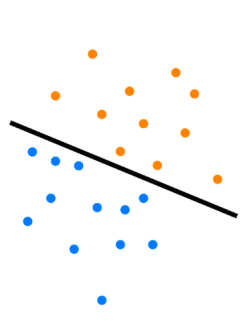
\includegraphics[scale=0.37]{Classified.png}
   	\caption{A separating line that can help classify our data}
\end{figure}

\pagebreak
\section{Logistic Regression (Single Neuron Classifier)}
We restrict our hypothesis class to linear separators (hyperplanes) and, given an input $x \in \mathbb{R}^n$, compute $a = \sum_{i=0}^{n}w_ix^i$.
Here the vector $w \in \mathbb{R}^n$ is our classifier and $x^i$ is the i-th component of the vector $x$.


The quantity $a$ is then sent through a function whose output we use to classify the input $x$.
\\
Some candidate functions are:
\begin{enumerate}
\item $y(a) = a$
\item $y(a) = \frac{1}{1+e^{-a}}$
\item $y(a) = sign(a)$
\end{enumerate}

Pictorially, this process can be represented as a neuron in the following manner.

\begin{figure}[H]
	\centering
		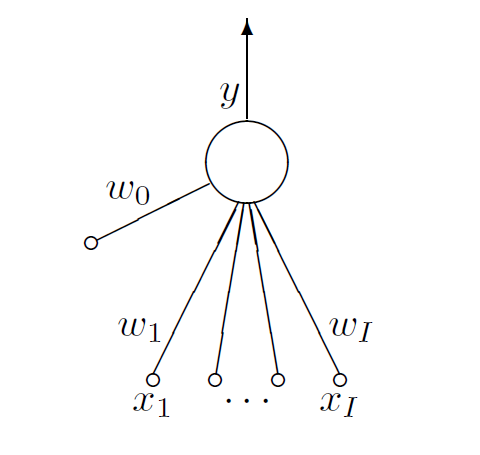
\includegraphics[scale=0.56]{SingleNeuron.PNG}
   	\caption{A single neuron}
\end{figure}

Why do people choose $y(a) = \frac{1}{1+e^{-a}}$?
This function, called the logistic function, has the disadvantage that it is hard to compute digitally. It's advantage is that it is analytically nice and smooth.
\\
But the key reason is that using it allows us a nice interpretation of the neuron via physics.
\\ \\
\textbf{Physics Interpretation to the Logistic function:}
Suppose there is a 2-state neuron. The state "Yes" has energy E and the state "No" has energy 0.
If $E(Yes) =-\sum_{i=0}^nw_ix^i$ and E(No) = 0.
\\ \\
Then from thermodynamics we would expect $P(Yes|E) \propto e^a$ and $P(No|E) \propto e^0$.
\\ \\
This would give us $Pr(Yes) = \frac{e^a}{1+e^a} = \frac{1}{1+e^{-a}}$.
Hence we can interpret this as the energy barrier for neurons firing. The probability of the neuron firing changes with change in $a$.
\\ \\
Of course, the actual neuron in the brain is much more complicated and this is merely a very simplified toy model that is nevertheless useful in providing intuition when we consider many neurons together.

\section{Error Model}
We want to choose the weights $w$ that minimize the error according to some error model. We now present an error model that can be interpreted both information-theoretically as well as statistically.

$$G(w) = -\sum_{i=1}^N[t_ilog(y(x_i;w))+(1-t_i)log(1-y(x_i;w))]$$

This can be interpreted as the total expected surprise from the data given our prior belief $w$. Hence minimizing this quantity seems reasonable. This is the information theoretic interpretation.

This quantity can also be seen as the negative log-likelihood of the data. Hence minimizing it is the same as maximizing the likelihood.
\\ \\
As a function of $w$, $G(w)$ need not be convex. However, the easiest thing we can do is gradient-descent and obtain a local optima. We shall see that gradient descent for this particular error model has a nice interpretation.

\textbf{Gradient Descent:}
$$\frac{\partial G}{\partial w_j} = -\sum_{i=1}^N[(t_i-y_i)x_i^j]$$
The error decreases in the direction of the negative of the gradient.
Hence we pick a learning rate and move in the direction opposite to the gradient in w-space.
\\ \\
This is called Hebbian Learning. It has the nice interpretation that if some input coordinate (say $x^j$) was right and we did not listen to it, it's contribution in the weights is increased ($w_j$ increases). Similarly if some input is wrong but we gave it large weight, we reduce its contribution.

\textbf{Remarks on Hebbian Learning:}
\begin{enumerate}
\item If the data points are linearly separable, after some time, Hebbian learning does not converge but diverges and all the weights go to $\infty$. This means the sigmoids become sharper and sharper but this may not lead to any actual decrease in prediction error. Hence this is false refining.
\item People counter this in different ways. Some just stop the algorithm after a while, even though it has not converged. This is called early stopping.
\item Some add a regularizing term ($\lambda ||w||^2$) corresponding to the weight of $w$ to the error function being optimized. This means that weights of $w$ won't increase too much unless there is a significant gain associated with it.
\end{enumerate}

\end{document}
